\ifdefined\cheatsheetCompact
  \documentclass[8pt]{extarticle}
  \usepackage[a4paper,xetex,landscape,left=1cm,right=1cm,
              top=0.7cm,bottom=0.7cm]{geometry}
\else
  \documentclass[12pt]{extarticle}
  \usepackage[a4paper,xetex,top=1.5cm,bottom=2cm]{geometry}
\fi

\usepackage{titlesec}

\titleformat{\section}
  {\normalfont\sffamily\large\bfseries\color{blue}}
  {\thesection}{1em}{}

\titleformat{\subsection}
  {\normalfont\sffamily\bfseries\color{blue}}
  {\thesubsection}{1em}{}

\titleformat{\subsubsection}
  {\normalfont\sffamily\small\bfseries\color{blue}}
  {\thesubsubsection}{1em}{}

\usepackage{calc}

\ifdefined\cheatsheetCompact
\usepackage{multicol}

% Compact titles %%%%%%%%%%%%%%%%%%%%%%%%%%%%%%%%%%%%%%%%%%%%%%%%%%%%%%

\titlespacing*{\section}
{-1.2ex}{0ex}{0ex}
\titlespacing*{\subsection}
{-1.2ex}{0ex}{0ex}
\titlespacing*{\subsubsection}
{-1.2ex}{0ex}{0ex}

\raggedcolumns

% Don't print section numbers
\setcounter{secnumdepth}{1}

% no space before new paragraph
\setlength{\parindent}{0pt}
\setlength{\parskip}{0pt}

% less spacing between items
\usepackage{enumitem}

\setlist[enumerate]{
    labelindent=25pt,
    leftmargin=*,
    itemsep=-0.2em
}
\setlist[itemize]{
    labelindent=25pt,
    leftmargin=*,
    itemsep=-0.2em
}

% Turn off header and footer
\pagestyle{empty}
 
\newcommand{\vshort}[1]{%
\vspace{-0.6em}%
#1%
\vspace{-0.3em}}

\else

\newcommand{\vshort}[1]{%
#1%
}

%\newcommand{\sectionbreak}{}

\fi

%%%%%%%%%%%%%%%%%%%%%%%%%%%%%%%%%%%%%%%%%%%%%%%%%%%%%%%%%%%%%%%%%%%%%%%

\usepackage{tabulary}
% make tabulary prevent overflows (https://tex.stackexchange.com/a/195088)
\tymin=60pt
\tymax=\maxdimen

\usepackage[table,usenames,dvipsnames]{xcolor}
\usepackage{adjustbox}
\usepackage[most]{tcolorbox}
\usepackage{fontspec}
\usepackage[urlbordercolor=blue,linkbordercolor=cyan,
            pdfborderstyle={/S/U/W 1}]{hyperref}

% declare font faces for Nunito font https://fonts.google.com/specimen/Nunito
% I don't use package `nunito` since it's not present in older Linux boxes,
% but instead download directly. Also in my installation presence of
% Nunito-VariableFont_wght.ttf/Nunito-Italic-VariableFont_wght.ttf broke
% some font shapes finding so I deleted it leaving only "static" ttf fonts.

\usepackage{fourier} % for \warning
\newcommand{\mywarning}{{\huge \warning}}

\setmainfont{Nunito}[
    FontFace={el}{n}{Font=* ExtraLight},
    FontFace={l}{n}{Font=* Light},
    FontFace={r}{n}{Font=*},
    FontFace={m}{n}{Font=* Medium},
    FontFace={sb}{n}{Font=* SemiBold},
    FontFace={b}{n}{Font=* Bold},
    FontFace={eb}{n}{Font=* ExtraBold},
    FontFace={xb}{n}{Font=* Black},
    FontFace={eli}{i}{Font=* ExtraLight Italic},
    FontFace={i}{i}{Font=* Italic},
    FontFace={mi}{i}{Font=* Medium Italic},
    FontFace={sbi}{i}{Font=* SemiBold Italic},
    FontFace={bi}{i}{Font=* Bold Italic},
    FontFace={ebi}{i}{Font=* ExtraBold Italic},
    FontFace={xbi}{i}{Font=* Black Italic},
]

\DeclareRobustCommand{\elseries}{\fontseries{el}\selectfont}
\DeclareRobustCommand{\lseries}{\fontseries{l}\selectfont}
\DeclareRobustCommand{\rseries}{\fontseries{r}\selectfont}
\DeclareRobustCommand{\mseries}{\fontseries{m}\selectfont}
\DeclareRobustCommand{\sbseries}{\fontseries{sb}\selectfont}
\DeclareRobustCommand{\bseries}{\fontseries{b}\selectfont}
\DeclareRobustCommand{\ebseries}{\fontseries{eb}\selectfont}
\DeclareRobustCommand{\xbseries}{\fontseries{xb}\selectfont}
\DeclareRobustCommand{\eliseries}{\fontseries{eli}\fontshape{i}\selectfont}
\DeclareRobustCommand{\liseries}{\fontseries{li}\fontshape{i}\selectfont}
\DeclareRobustCommand{\iseries}{\fontseries{i}\fontshape{i}\selectfont}
\DeclareRobustCommand{\miseries}{\fontseries{mi}\fontshape{i}\selectfont}
\DeclareRobustCommand{\sbiseries}{\fontseries{sbi}\fontshape{i}\selectfont}
\DeclareRobustCommand{\biseries}{\fontseries{bi}\fontshape{i}\selectfont}
\DeclareRobustCommand{\ebiseries}{\fontseries{ebi}\fontshape{i}\selectfont}
\DeclareRobustCommand{\xbiseries}{\fontseries{xbi}\fontshape{i}\selectfont}

% redefine default bold to extra bold
\DeclareRobustCommand{\bfseries}{\fontseries{eb}\fontshape{n}\selectfont}
% fix \textit
\DeclareTextFontCommand{\textit}{\iseries}

% font for headings
\setsansfont{Open Sans}

% some bolder font
\usepackage{unicode-math}
\setmathfont[Scale=1.0]{TeX Gyre Schola Math}

\usepackage{circledsteps}  % for \Circled
\pgfkeys{/csteps/inner color=white}
\pgfkeys{/csteps/outer color=black}
\pgfkeys{/csteps/fill color=black}
\newcommand{\circled}[1]{\Circled{\textbf{#1}}}

\usepackage{tikz}
\usetikzlibrary{shapes,arrows,positioning,calc,fit}
\tikzset{
block/.style = {draw, fill=white, rectangle, minimum height=3em, minimum width=3em},
line/.style={-latex},
}

% definition for drawing arrow
\newcommand{\tikzmark}[1]{\tikz[overlay,remember picture] \node (#1) {};}
\newcommand{\DrawBottomReverse}[2]{%
  \begin{tikzpicture}[overlay,remember picture,-latex,shorten >=5pt,shorten
      <=5pt,out=225,in=315]
      \draw[distance=0.45cm,#1] (a.south) to node[right,xshift=1.1cm]{#2}
      (b.south);
  \end{tikzpicture}
}

\newtcolorbox{prebox}[1][]{
    left=0.5mm, right=0.5mm, top=0mm, bottom=0mm,
    before skip=3pt, after skip=3pt,
    frame hidden, boxrule=0.05em,
    colback=green!10, #1}

% colored box around code
\newenvironment{code}[1][]{%
\begin{prebox}[#1]\obeylines%
\fontdimen2\font=0.9ex% inter word space
}{%
\end{prebox}%
\fontdimen2\font=0.6ex% inter word space
}

% box with modifiable size
\newenvironment{codem}[2][\linewidth]{%
\begin{minipage}{#1}%
\begin{prebox}[colback=#2]\obeylines}{%
\end{prebox}%
\end{minipage}}

% box with size 90%
\newenvironment{code9}{%
\begin{codem}[0.9\linewidth]{green!10}}{\end{codem}}

% inline color box for code
\newcommand{\cod}[2][green!10]{\tcbox[
    size=fbox,
    on line,
    colback=#1,
    colframe=black,
    arc=0.3em  % rounded corners
]{#2}}

% Syntax highlighting for code %%%%%%%%%%%%%%%%%%%%%%%%%%%%%%%%%%%%%%%%
\newcommand{\ind}{\hphantom{~~~}}
% shell and other prompts
\newcommand{\prompt}{\textcolor{red}{\textbf{\$}\ }}
% target prompt:
\newcommand{\tprompt}{\textcolor{brown}{\textbf{target\$}\ }}
\newcommand{\sprompt}{\textcolor{blue}{\textbf{>}\ }}
% Syntax:
\newcommand{\kw}[1]{\textcolor{magenta}{\textbf{#1}}}
\definecolor{myOrange}{rgb}{0.7,0.25,0}
\newcommand{\ty}[1]{\textcolor{myOrange}{\textbf{#1}}}
% Misc highlighting:
\newcommand{\hl}[1]{\textcolor{blue}{\textbf{#1}}}
% shell/simics script/python comment
\newcommand{\cmtcommon}[1]{\textcolor{Sepia}{\textbf{#1}}}
\newcommand{\cmt}[1]{\cmtcommon{\#\ #1}}
% DML/C comment:
\newcommand{\cmtd}[1]{\cmtcommon{/\,/\ #1}}
\newcommand{\p}[1]{\textit{\large#1}}
%%%%%%%%%%%%%%%%%%%%%%%%%%%%%%%%%%%%%%%%%%%%%%%%%%%%%%%%%%%%%%%%%%%%%%%

\fontdimen2\font=0.6ex% inter word space

% This document specific declarations %%%%%%%%%%%%%%%%%%%%%%%%%%%%%%%%%
\newcommand{\local}{\kw{local} }
\usepackage{underscore}  % underscore is often used in code here
\newcommand{\Simics}{\textcolor{cyan}{\textbf{Simics}}}

\newlength{\connectwidth}
\ifdefined\cheatsheetCompact
\setlength{\connectwidth}{3cm}
\else
\setlength{\connectwidth}{5cm}
\fi
\newlength{\MyLen}
%%%%%%%%%%%%%%%%%%%%%%%%%%%%%%%%%%%%%%%%%%%%%%%%%%%%%%%%%%%%%%%%%%%%%%%

\begin{document}

% Never allow text overflow to margin:
\setlength\emergencystretch{\hsize}\hbadness=10000


\ifdefined\cheatsheetCompact
\begin{multicols*}{3}
\fi
    {\Large\centering \Simics{} Cheatsheet\par}
    %\section*{Simics cheatsheet}
    %\begin{center} \textbf{\Large \Simics{} Cheat Sheet} \end{center}

\ifdefined\cheatsheetCompact
\vspace{0.2cm}
\fi

\section{\Simics{} Usage (command line)}

\subsection{Glossary \& Documentation}
    \settowidth{\MyLen}{\textit{[simics]-script.}}
    \rowcolors{1}{gray!15}{white}
    \noindent\begin{tabular}{p{\the\MyLen}p{\linewidth-\the\MyLen-0.8cm}}
        \textit{\Simics{} Base} & \cod{simics} executable + the set of
        supporting shared libraries (DLLs) + tools
        \\
        \textit{simulation}  & running of code (target) on
        a model/platform (target) with advancement of time
        \\
        \textit{host}        & a computer where simulation runs
        \\
        \textit{target}      & a simulated
        code running in its isolated memory region, e.g. Linux or
        Windows guest
        \\
        \textit{platform}  & a complete runnable model:
        full set-up of devices
        with CPU or with at least a clock provider
        \\
        \textit{package}   & a set of devices, oftentimes constituting
        1 platform, distributed as a whole in an archive and unpacked
        into 1 directory
        \\
        \textit{[\Simics] Script} & simple Unix-shell-like language (a wrapper
        over Python) used for connecting devices and command line 
        automation
        \\
        \textit{Simics User’s Guide} & documentation on \Simics{}
        usage — both command line and Eclipse
    \end{tabular}

    Below \prompt stands for Unix shell prompt, \sprompt for \Simics{} prompt.
    \p{Big_italic} text means user-supplied arguments for commands/functions.

\subsection{Getting help}
\begin{code}
    \cmt{Get help on some command:}
    \sprompt{help \p{instantiate-components}}
    \cmt{Finding sections of documentation mentioning it:}
    \sprompt{apropos \p{instantiate-components}}
\end{code}

\subsection{Set up a workspace with platform package}
    \begin{code}
        \prompt \p{path/to/simics-base}/bin/project-setup\ \ .
        \prompt bin/addon-manager -c  \cmt{remove default package associations}
        \cmt{allow scripts \& shared libraries be found:}
        \prompt bin/addon-manager -s /path/to/platform-package
        \prompt bin/addon-manager -s /path/to/additional/package
    \end{code}

\subsection{Start up}
    \begin{code}
        \prompt ./simics targets/\p{platf/platf.simics}
    \end{code}

    
    %\begin{tabular}{|p{6cm}| p{10cm} |}
    Shell command line arguments $\longrightarrow$ \Simics{} command line 
        correspondence:

    \noindent\begin{tabular}{p{0.05\linewidth}p{0.85\linewidth}}
        &
        \begin{code9}
            \prompt ./simics start.simics
        \end{code9}
        \vspace{0.05cm}
        \\
        $\longrightarrow$ &
        \begin{code9}
            \prompt ./simics
            \sprompt run-command-file start.simics
        \end{code9}
        \vspace{0.2cm}
        \\

        & \begin{code9}
            \prompt ./simics script.py
        \end{code9}
        \vspace{0.05cm}
        \\
        $\longrightarrow$ &
        \begin{code9}
            \prompt ./simics
            \sprompt run-python-file script.py
        \end{code9}
        \vspace{0.2cm}
        \\

        & \begin{code9}
            \prompt ./simics -e ‘\$config_variable1=value; \$config_var2=value’ start.simics

            \cmt{\mywarning NOT ./simics start.simics -e \$varibables ...}
        \end{code9}
        \vspace{0.05cm}
        \\
        $\longrightarrow$ &
        \begin{code9}
            \prompt ./simics
            \sprompt \$config_variable=value
            \sprompt \$config_var2=value
            \sprompt run-command-file start.simics
        \end{code9}
    \end{tabular}

\subsection{Environment \& Packages}
    \begin{code}
        \sprompt version  \cmt{list of installed packages}
        \prompt ./simics -v \cmt{the same}
        \sprompt pwd \cmt{current directory where simics is running}
        \sprompt list-directories \cmt{where \Simics{} searches files}
    \end{code}


    To debug chain of called auxiliary scripts \cod{include}s:
    \begin{code}
        \prompt ./simics -script-trace targets/\p{platf/platf.simics}
    \end{code}

\subsection{Commands for running simulation}
\begin{code}
\sprompt c[ontinue]
\sprompt r[un] 100 cycles \ind \cmt{or 10 steps or 0.1 seconds}
\sprompt ptime [-all] \ind \cmt{to show target's time}
\end{code}

\subsection{Printing device structure}
To find devices by name/class or interface name:
    \begin{code}
        \sprompt list-objects -all \p{name} \ind \cmt{searches also for the class}
        \sprompt list-objects -all substr = \p{mem} \cmt{object names containing \p{mem}}
        \sprompt list-objects -all iface = \p{my_interface} \cmt{by interface name}
    \end{code}

To examine device structure (\Simics{} \textit{components}
and \textit{devices}) of a given component \p{myPlatform}:
\begin{code}
    \cmt{1-level representation: immediate children \p{myPlatform}:}
    \sprompt list-objects namespace = \p{myPlatform}
    \cmt{multi-level one: all children of \p{myPlatform} with all hierarchy:}
    \sprompt list-objects namespace = \p{myPlatform} -tree
\end{code}

To find all objects with the same class as given device:
        \begin{code}
            \begin{code}
            \sprompt \p{platf.myDevice}->classname
            \p{my_class}
            \end{code}
            \sprompt list-objects -all \p{my_class}
            \sprompt list-objects -all class = \p{my_class}
        \end{code}

\subsection{Registers}
\begin{code}
    \cmt{print all registers:}
    \sprompt print-device-regs \p{platf.myDevice}
    \cmt{print fields of register \p{myRegister}:}
    \sprompt print-device-reg-info \p{platf.myDevice.myBank.myRegister}
\end{code}

\subsubsection{Writing/reading with side effects}

\begin{code}
    \sprompt write-device-reg
    \ind \ind \p{platf.myDev}.bank.\p{myBank.myGrp.myReg} 0x1
    \cmt{(Register groups like \p{myGrp} may be omitted in devices)}
    \sprompt read-device-reg \p{platf.myDev}.bank.\p{myBank.myGrp.myReg}
\end{code}

%\subsubsection{Writing/reading \textbf{without} side effects (aka set/get)}
\subsubsection{Writing/reading {\bseries without} side effects (aka set/get)}

It's done through attributes:
\begin{code}
    \cmt{To set to value 0x1}
    \p{platf.myDev}->\p{myBank_myGrp_myReg} = 0x1
    \cmt{To get the value:}
    \p{platf.myDev}->\p{myBank_myGrp_myReg}
\end{code}

\subsection{Connects — attributes that point to other devices}

\begin{code}
    \cmt{to set connect attribute:}
    \sprompt \p{platf.myDevice}->\p{myConnect} = "\p{platf.anotherDevice}"
    \cmt{to zero connect attribute:}
    \sprompt \p{platf.myDevice}->\p{myConnect} = FALSE \ind\cmt{obvious ;-)}
\end{code}

\subsection{Device information: static}

\begin{code}
    \cmt{To find info about class/module/package for your device:}
    \begin{code}
    \sprompt help \p{platf.myDev}
    \ind Class \textbf{myClass}
    \vspace{0.3em} \ind Provided By
    \ind \ind   \textbf{myModule} (from \textbf{myPackage})
    \vspace{0.2em}
    \ind \cmt{...then documentation about the device is printed.}
    \end{code}
    \vspace{0.3em}

    \cmt{To list all classes provided by a module:}
    \sprompt list-classes -m \p{myModule}
    \cmt{Configuration information}
    \sprompt \p{platf.myDev}.info
\end{code}

\subsection{Device information: dynamic}

\begin{code}
    \cmt{Runtime information:}
    \sprompt \p{platf.myDev}.status
    \cmt{pretty-print device attributes with values:}
    \sprompt list-attributes \p{platf.myDev}
    \cmt{to search all attributes/registers containing \p{mem}:}
    list-attributes \p{platf.myDevice} substr = \p{mem}
\end{code}


\subsection{Debugger commands}
To use \Simics{} to debug target:
\begin{code}
dis[assemble] \cmt{show assembler commands at current address}

\cmt{Break points:}
break address
break-hap Core-Magic-Instruction
\end{code}

\subsection{Memory spaces}

All target software runs on CPU and can access devices only through
hierarchy of memory spaces:

\noindent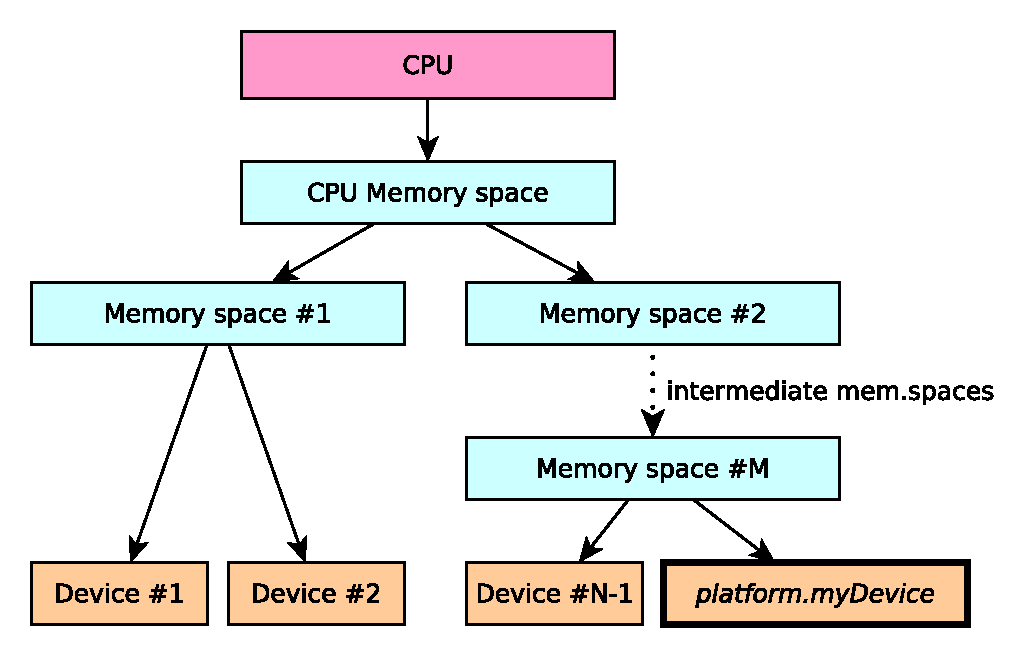
\includegraphics[width=\linewidth]{diagrams/mem_spaces.pdf}

\begin{code}
    \cmt{To find memory spaces the device is mapped in:}
    \sprompt devs \p{platf.myDevice}
\end{code}

\subsection{Examining current state}

\noindent\begin{tabular}{ll}
    pselect & show currently running CPU \\
    memory-map & print all mapped devices \\
    pregs & print all CPU registers \\
    probe-address \p{addr} & path to target \p{addr}
\end{tabular}

\subsection{x86-specific and platform-specific commands}

\noindent\begin{tabular}{ll}
    memory-trace \p{addr} & path to target \p{addr} \\
    pregs & to know x86 mode (16/32/64-bit), 1st line \\
    reset-button-press & to reboot the target \\
    power-button-press & to press power button \\
\end{tabular}


\subsection{Moving files target \texorpdfstring{$\longleftrightarrow$}{<->} host}
%\subsection{Moving files target $\longleftrightarrow$ host}
%\subsection{Moving files target <-> host}
\begin{code}
\sprompt start-simicsfs-server
\end{code}

\begin{code}[colback=blue!15]
\tprompt mkdir a
\tprompt simicsfs-client a
\end{code}

\subsection{Saving info}
Save logs from current point
\begin{code}
    \sprompt start-command-line-capture \p{filename}
\end{code}

Save simics variables to file
\begin{code}
    \sprompt start-command-line-capture \p{filename}
    \sprompt list-variables
    \sprompt stop-command-line-capture
\end{code}

\subsection{Check points}
\noindent\begin{tabular}{ll}
            \cod{write-configuration \p{"checkpoint_name"}} & — save
            checkpoint \\
            \cod{read-configuration \p{"checkpoint_name"}} & — restore it back
\end{tabular}

%\subsection{Making images}

\subsection{Miscellaneous}
\begin{code}
    \cmt{To dump network packages (for analysis with Wireshark)}:
    \sprompt pcap-dump link=\p{ethernet_switch0} filename=\p{myFile}
    \begin{code}
    \cmt{Treat all input as Python code}
    \sprompt python-mode
        \sprompt \sprompt \sprompt \p{Enter your code}
    \end{code}
    
\end{code}

\ifdefined\cheatsheetCompact
% \newpage
\vspace{0.4cm}
\fi

\section{\Simics{} DML 1.4 Programming \& C/DML API}

\subsection{Glossary \& Documentation}
    \settowidth{\MyLen}{\texttt{dml-1.4-reference-man}}
    %\begin{tabulary}{\linewidth}{p{4cm}L}
    \noindent\begin{tabular}{p{\the\MyLen}p{\linewidth-\the\MyLen-0.8cm}}
        \textit{DML}         & Device Modelling Language is a
        wrapper over C for writing (fast) devices.
        Its compiler is included into \Simics{} Base.
        \\
        \kw{device}          & any \Simics{} class for modelling real
        devices. Different \Simics{} devices communicate via \textit{interfaces}.
        \\
        \textit{Model Builder User’s Guide} & overview of \Simics{}/DML
        programming \\
        \textit{DML 1.4 Reference Manual} & language specification \\
        \textit{API Reference Manual} & API function list for DML \& C,
        describes ownership rules\\
        \textit{model writers} & those who write \Simics{} devices\\
        \textit{users} & those who use \Simics{} devices:
                         device driver writers, firmware/UEFI writers,
                         validators/testers, etc
    \end{tabular}

\subsection{Getting help}
\begin{code}
    \cmt{Print explanation of C/Python/DML API functions:}
    \sprompt api-help \p{SIM_add_configuration}
\end{code}

\subsection{Create stub device}

\begin{code}
    \prompt bin/project-setup -{}-device \p{example-dev}
    \prompt ls modules/\p{example-dev}
    test/  \p{example-dev}.dml  Makefile  module_load.py
\end{code}

The header of \p{example-dev}.dml is then:

\begin{code}
    %\begin{tabulary}{\linewidth}{p{4cm}L}
    %\begin{tabular}{p{3cm}p{\linewidth-3.8cm}}
    \rowcolors{1}{}{}
    \noindent\begin{tabular}{ll}
        dml 1.4;                  & \cmtd{Obligatory .dml header} \\
        \kw{device} \p{example_dev};  & \cmtd{Class name.} \\
                                  & \cmtd{Note: - changed to underscore _}
    \end{tabular}
\end{code}

\subsection{Create stub interface with Python wrapper}

\begin{code}
    \prompt bin/project-setup -{}-interface \p{sample}
    \prompt ls modules/\p{sample}-interface
    Makefile  \p{sample}-interface.dml  \p{sample}-interface.h
\end{code}

Python support is enabled by \cod{IFACE_FILES} in the Makefile.
The generated C \kw{struct} name is \cod{\ty{\p{sample}_interface_t}}.

\subsection{Arithmetics}

\subsubsection{RHS is int64, LHS truncates}

Assignments are equivalent to casts and hence can truncate:
        \begin{code}
            \local \ty{uint8} x = 0xffff  \cmtd{results in x == 0xff}
        \end{code}

        All aritmetic operators like $+$, $*$ convert its operands to int64:
        \begin{code}
            \local \ty{uint16} $i$ = 0x7fff; \local \ty{int8} $j$ = 2;  \cmtd{let us sum them:}
            \vspace{0.1cm}
            \local \ty{int16} \tikzmark{b} $x$ = $\overbrace{\ind i + j; \ind }^{\text{calculates as \ty{int64} $\rightarrow$ 0x8001} \tikzmark{a}}$ \DrawBottomReverse{black}{truncates to \ty{int16}}
            \vspace{0.3cm}
            \cmtd{finally results in $x == 1$}
        \end{code}


\subsubsection{Comparisons act as uint64 or int64: $==$, $<$, $<=$}
Comparisons on only uint64 act as proper uint64, however
in comparisons int64 vs. uint64 the operands are converted to int64!

        \begin{code}
            \local \ty{uint64} u;
            u = -1; \ind \cmtd{equivalent to u = cast(-1, uint64) $\mathbf{= 2^{64}-1}$, all ones}
            \rowcolors{1}{}{}
            \noindent\begin{tabular}{@{}ll}
                u == -1 & \cmtd{FALSE! Equivalent to int64(u) == int64(-1),} \\
                        & \cmtd{where upper bit is cropped: int64(u) == ($\mathbf{2^{63}-1}$).}
            \end{tabular}
            u == cast(-1, \ty{uint64}) \cmtd{true. As comparison is b/w two uint64}
            u > -1 \ind \cmtd{true, but unlike C! it's int64(u) > int64(-1): $\mathbf{2^{63}-1>1}$}
        \end{code}

\subsection{Syntax}

    \subsubsection{Statements}
    \begin{code}
        \cmtd{Printing through \kw{log} statements:}
        \kw{log} \p{log-type}, $\underbrace{level}_{\makebox[0pt]{\text{default 1\hspace{0.5cm}}}}$, $\underbrace{groups}_{\makebox[0pt]{\hspace{1.7cm}\text{default 0 (no group)}}}$: \p{"format-string"}, $arg_1$, ..., $arg_N$;
        \cmtd{(The "format-string" is the same as in C, see `man 3 printf')}
    \end{code}
    \global\rownum=0\relax
    \noindent\begin{tabulary}{\linewidth}{|LL|}
        \hline
        \p{log-level} & usage rule \\
        \hline
        1 & most important messages (for both users and model writers),
            typically \texttt{error}\\
        2 & crucial events for boards/devices, e.g. their resets \\
        3 & any other messages (for users) \\
        4 & internal device debug messages (for model writers)\\
        \hline
    \end{tabulary}
    \noindent\begin{tabulary}{\linewidth}{|LL|}
        \hline
        \p{log-type} & usage rule \\
        \hline
        \texttt{info} & informational message \\
        \texttt{spec_viol} & specification violation by target software (for users) \\
        \texttt{unimpl} & attempt to use not implemented functionality (for users) \\
        \texttt{error} & internal device error (for model writers).
                \mywarning There is a limit (default 10_000) after
                which simulation stops!\\
        \texttt{critical} & like \texttt{spec_viol} or error, but \mywarning
                   stops simulation \\
        \hline
    \end{tabulary}
    \begin{code}
        \cmtd{Dynamic allocation (like malloc() in C):}
        \local \ty{$type$ *} x = \kw{new} \ty{$type$};
        \cmtd{e.g. for int array:}
        \local \ty{int *} x = \kw{new} \ty{int[100]};
        \kw{delete} x;  \cmtd{Deallocation like free() in C}
        \cmtd{Raising/catching exceptions:}
        \kw{try} \{
            \ind \kw{throw;}  \cmtd{YES, no data can be carried by exception}
        \} catch \{
            \vshort{\ind ...}
        \}
    \end{code}

    \subsubsection{Expressions}
    \begin{code}
        sizeof $value$  \cmtd{: int — get byte size of the value}
        sizeoftype \ty{$type$}  \cmtd{: int — get byte size of the type}
        x[10:8]  \cmtd{Get bits 10—8 of integer $x$:}
        x[8]  \cmtd{Get bit 8 of integer $x$:}
    \end{code}

    \subsubsection{Types}
    \ty{uint1}...\ty{uint64} and \ty{int1}...\ty{int64}.

    \subsubsection{Methods}
    They are called \textit{methods}, not functions, because
    they accept \textbf{implicit} 1st argument — object (current
    device), like C++ methods.
    \begin{code}
        \kw{method} \p{name}(\ty{$inputType_1$} $arg_1$) -> (\ty{$outputType_1$}, \ty{$outputType_2$}) \{
            \vshort{\ind ...}
            \ind \kw{local} \ty{$outputType_1$} $var_1$ = ...; \kw{local} \ty{$outputType_2$} $var_2$ = ...;
            \ind return $(var_1, var_2)$;
        \}
        \cmtd{calling this method:}
        \kw{local} \ty{$inputType_1$} val = ...;
        \kw{local} \ty{$outputType_1$} x; \kw{local} \ty{$outputType_2$} y;
        (x, y) = \p{name}(val);
    \end{code}

    \subsubsection{Bitfields}
    \begin{code}
        bitfields 32 \{
            \ind \ty{uint3} \p{upper_bits} @ [31:29];
            \vshort{\ind ...}
        \}
    \end{code}

    \subsubsection{Object declarations}
    \begin{code}
        \p{objectType} \p{objectName} \{
            \ind \kw{method} \p{methodName} \{
            \ind     \vshort{\ind \ind ...}
            \ind \}
        \}
        register \p{regName} @ \p{offset} is ($template_1$, ...);
        \cmtd{@ \p{offset} is a syntax for "\kw{param} offset = \p{offset};"}
    \end{code}

\subsubsection{Module variables and other data objects}

    \global\rownum=1\relax
    \noindent\begin{tabulary}{\linewidth}{|LLLLL|}
        \hline
        DML construct & checkpointed & fields & address-mapped & arbitrary data\\
        \hline
        \kw{session} & - & - & - & + \\
        \kw{saved} & + & - & - & - \\
        attribute & + & - & - & + \\
        unmapped register & + & + & - & - \\
        {[}normal{]} register & + & + & + & - \\
        \hline
    \end{tabulary}

    \subsubsection{Interfaces}

    Definition in \cod{.dml}:
    \begin{code}
        \kw{extern typedef struct} \{
            \ind \kw{method} \p{name}(\ty{conf_object_t *}\hl{obj}, \p{\ty{$type_1$} $value_1$})
            \ind \ind \ind -> \p{\ty{out_type}};
        \} \ty{\p{sample}_interface_t};
    \end{code}

    Obligatory definition in C \cod{.h} file \textbf{for using the interface from Python}:
    \begin{code}
        SIM_INTERFACE(\p{sample}) \{  \cmtd{essentially '\kw{typedef struct}' also}
            \ind \ty{\p{out_type}} (*\p{name})(\ty{conf_object_t *}\hl{obj}, \ty{\p{$type_1$}} \p{$value_1$});
        \}
        \#define \p{SAMPLE}_INTERFACE "\p{sample}" \ind \cmtd{necessary!}
    \end{code}

    Then it is called \textbf{without} \cod{\hl{obj}}: just \cod{\p{name}(\p{$value_1$})}.

    \subsubsection{Explaining \cod{connect}s and \cod[magenta!35]{implement}s}

    \begin{itemize}
        \item \cod{connect}s are for \textbf{out}bound calls
        \item \cod[magenta!35]{implement}s are for \textbf{in}bound calls
    \end{itemize}

    \noindent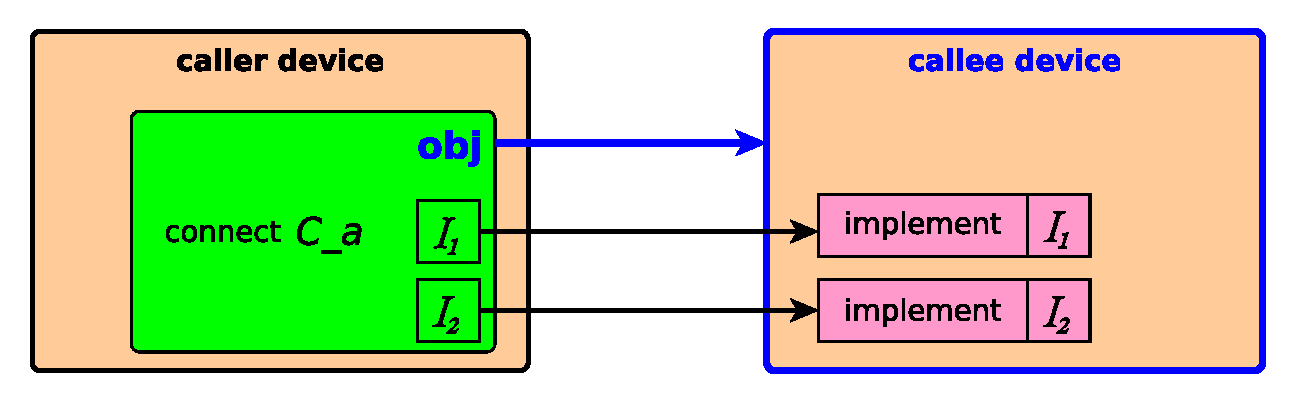
\includegraphics[width=\linewidth]{diagrams/connect_implement.pdf}

    \global\rownum=1\relax
    %\begin{tabulary}{\linewidth}{|LCC|}
    %\begin{tabular}{|lp{2.5cm}c|}
        \noindent\begin{tabular}{|lp{\connectwidth}p{\connectwidth}|}
        \hline
        %co & \begin{minipage}{2.5cm}unnamed (whole-device)\end{minipage} & 
         & unnamed (whole-device) & named (wrapped in attribute) \\
        \hline
        \cod{connect} & - &
            \begin{codem}[\connectwidth]{green!10}
                connect \p{C_a} \{ \circled{1}
                  \ind interface $I_1$ \{ \circled{2}
                      \vshort{\ind\ind ...}
                  \ind \}
                  \ind interface $I_2$ \{ \circled{2}
                      \vshort{\ind\ind ...}
                  \ind \}
                \}
                connect \p{C_b} \{  \circled{1}
                  \ind interface $I_2$ \{  \circled{2}
                    \vshort{\ind\ind ...}
                    %  \vspace{-0.6em}
                    %\ind\ind ...
            \end{codem}
            \\[1.4cm]  % selected by trial
        \cod[magenta!35]{implement} &
            %\begin{codem}[2.5cm]{magenta!35}
            \begin{codem}[\connectwidth]{magenta!35}
                implement $I_1$ \{
                    \ind ...
                \}
                implement $I_2$ \{
                    \ind ...
                \}
            \end{codem}
            (as in picture above)
            &
            \begin{codem}[\connectwidth]{magenta!35}
                port $P_A$ \{
                \ind implement $I_1$ \{
                    \vshort{\ind\ind ...}
                \ind\}
                \ind implement $I_2$ \{
                    \ind\ind \emph{... variant 1 ...}
                      \vspace{-0.3em}
                \ind\}
                \}
                port $P_B$ \{
                \ind implement $I_2$ \{
                    \ind\ind \emph{... variant 2 ...}
            \end{codem}
            \\
        \hline
    \end{tabular}
    %\end{tabulary}

    \noindent\begin{tabulary}{\linewidth}{LL}
        \circled{1} & 
            \begin{minipage}{\linewidth}
                To make the whole \cod{connect} required:
                \begin{code}
                    \kw{param} configuration = "required";\\
                    \cmtd{other variants: "optional" (default), "pseudo", "none"}
                \end{code}
            \end{minipage}
                \\
        \circled{2} & 
            Individual interfaces are already \textbf{required} by default, to make them optional:
                \begin{code}
                    \kw{param} required = false;
                \end{code}
    \end{tabulary}

\mywarning \cod[magenta!35]{implement \{\}} does NOT check that all (or any!) methods
of an interface are really provided, defaulting to \kw{NULL}.

\subsection{Calling device code from Python}

If \p{device} \cod{implement}s interface $iface_1$ then its methouds
can be invoked from \Simics{} command line via Python:
\begin{code}
    @conf.\p{platf.device}.iface.$iface_1$.$method_1$(\textit{argument_1}, ...)
\end{code}

\subsection{Debugging with Gdb}
To debug simics and its modules itself:
            %\cmt{Terminal \#1:}
        \begin{code}
            %\begin{center}Terminal \#1:\end{center}
            {\large\centering Terminal \#1:\par}
            \cmt{Recompile your module with debugging support:}
            \prompt make clobber-\p{my-module}
            \prompt make D=1 \p{my-module}
            \prompt ./simics
            \sprompt pid
            \p{12345}
        \end{code}

        \begin{code}[colback=blue!15]
            {\large\centering Terminal \#2:\par}
            \prompt bin/gdb
            >\,>\,> attach \p{12345}
            >\,>\,> br \p{file.dml:100}  \ind \cmt{set break point on line 100 of file.dml}
            >\,>\,> continue
        \end{code}

        \begin{code}
            {\large\centering Back to terminal \#1:\par}
            \sprompt run-command-file targets/\p{platf/platf.simics}
        \end{code}


\subsubsection{Using gdb for debugging target}
\begin{code}
    load-module gdb-remote
    new-gdb-remote \p{50000}  \ind \cmt{open port \p{50000}}
\end{code}


\subsection{Attribute values}
    \cod{\ty{attr_value_t}} is a C union that can hold one of a
    few predefined types.

    Attributes values are allocated/packed by:\\
    \cod{\ty{attr_value_t} x = \textbf{SIM_make_attr_\p{T}}(\ty{\p{cType}} val)},
    and extracted by:\\
    \cod{\ty{\p{cType}} \ind \ind val = \textbf{SIM_attr_\p{T}}(x)}, where
    \ty{\p{T}} and \ty{\p{cType}} can be:

        \global\rownum=0\relax
        \noindent\begin{tabulary}{\linewidth}{|LLL|}
            \hline
            \p{T}         & type spec & \p{cType} — DML/C type \\
            \hline
            uint64, int64 & i & \ty{uint64}, \ty{int64} \\
            boolean       & b & \ty{bool} \\
            floating      & f & \ty{double} \\
            string        & s & \ty{char*} \\
            object        & o & \ty{conf_object_t} \\
            list          & [\ty{$x_1$}...\ty{$x_n$}] & fixed-width tuple with $n$ elements of types \ty{$x_1$}, ..., \ty{$x_n$} \\
            list          & [\ty{$x$}*] & arbitrary-width array of \ty{$x$} \\
            list          & [$x+$] & non-empty arbitrary-width array
                                     of \ty{$x$} \\
            list          & [\ty{$x$}$\{m:n\}$] & array of \ty{$x$} with $m ≤ size ≤ n$ \\
            list          & [\ty{$x$}$\{n\}$] & fixed-width tuple with $n$
                                         elements of \ty{$x$} \\
            dict          & D & array of \ty{attr_dict_pair_t} \\
            data          & d & \ty{uint8*} \\
            nil           & n & \ty{void} or \ty{$x$*} \\
            invalid       &   &  (none, used for indicating errors) \\
            \hline
        \end{tabulary}

    List items are accessed by \cod{SIM_attr_list_item}.
    Type specs can be OR'ed as \cod{$x_1$\kw{|}$x_2$}.
    Type spec is used in \cod{\kw{param} type = "..."}. For first 4
    types there are predefined DML templates \cod{uint64_attr},
    \cod{int64_attr}, \cod{bool_attr}, \cod{double_attr}.

    \renewcommand\_{\textunderscore\linebreak[1]}

\subsection{Attribute initialization}
    \global\rownum=0\relax
    \noindent\begin{tabulary}{\linewidth}{|LLL|}
        \hline
        Execution stage & SIM_object_is_configured(obj) &
            SIM_is_restoring_state(\,) \\
        \hline
        Create object at 1st platform init & - & - \\
        Load checkpoint & - & + \\
        Load micro-checkpoint (reverse execution) & + & + \\
        Manual attribute assignment (hot plug from \Simics{} command line) & + & - \\
        \hline
    \end{tabulary}

\subsection{Standard register templates}

\subsection{Compile-time statements \& conditional compilation}

\begin{code}
    \kw{param} \p{p1} = 10; \cmtd{Non-overridable parameter}
    \kw{param} \p{p2} default "value"; \cmtd{Overridable parameter}
    template \p{myTemplate} \{
        \ind param \p{p3}; \cmtd{undefined value — must be given on \p{myTemplate} instantiation}
        \vshort{\ind ...}
    \}
    \cmtd{Compile-time \kw{if}}
    \kw{\#if} (p1 == 20) \{
        \vshort{\ind ...}
    \} \kw{\#else \#if} \{
        \vshort{\ind ...}
    \} \kw{\#else} \{
        \vshort{\ind ...}
    \}
    \cmtd{Compile-time ternary operator \kw{\#?} \kw{\#:}}
    param mode = p1 == 20 \kw{\#?} "equal 20" \kw{\#:} "not equal 20";
    \cmtd{Represent \textit{value} of parameter as string}
    param p1_str = stringify(p1);  \cmtd{results in "10"}
\end{code}


\subsection{Hash tables}

        \begin{code}
            \kw{import} "simics/util/hashtab.dml";
            \vshort{...}
            \local \ty{ht_str_table_t} tab;  \cmtd{str — string (aka const char*) keys.}
            ht_init_str_table(\kw{\&}tab, \cmtcommon{/*keys_owned*/} true);
            \local \ty{double *}value = new \ty{double};  \kw{*}value = 10.0;
            ht_insert_str(\kw{\&}table, "key", cast(value, \ty{void *}));
            \local \ty{double *}get_back = cast(ht_lookup_str(\kw{\&}tab, "key"), \ty{double*});
            assert \kw{*}get_back == 10.0;
        \end{code}
        There are also tables for \cod{\ty{int}} keys or general (\cod{common}) keys.

\subsection{The secret of DML}
        Many "internal" features like registers and even connects are actually
        normal templates for objects (\cod{\kw{is} object;}) in plain DML
        defined in \texttt{1.4/dml-builtins.dml} and thus they can be expanded.

\subsection{C API}

It's possible to do most things in C, e.g. create device by
\cod{SIM_create_object}, though normally it's done from Python components.

\ifdefined\cheatsheetCompact
\vspace{0.4cm}
% \newpage
\fi


\section{\Simics{} configuration and build system}

\subsection{Glossary \& Documentation}
    \settowidth{\MyLen}{\texttt{Components}}
    %\begin{tabulary}{\linewidth}{p{4cm}L}
    \noindent\begin{tabular}{p{\the\MyLen}p{\linewidth-\the\MyLen-0.8cm}}
        \textit{Python}      & this language is used for connecting 
        devices together (writing components), for writing
        some (slow) devices, for unit-testing
        \\
        \textit{Component}  & a special \Simics{} class that 
        forms a namespace tree and (typically) in its nodes
        contains instances of device classses. Components implement
        required \cod{component} interface and
        optional \cod{component_connector} interface.

    \end{tabular}

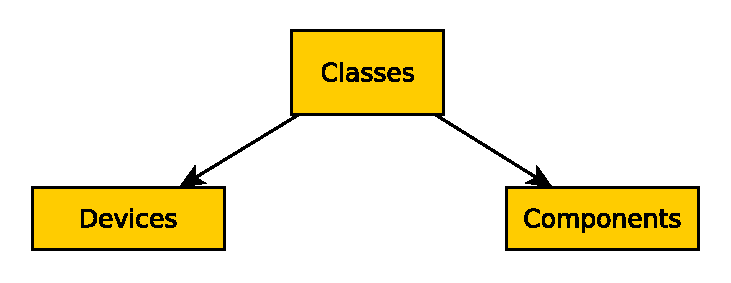
\includegraphics[width=\linewidth]{diagrams/classes_devices_components.pdf}
\subsection{Creating devices dynamically}
\begin{code}
\sprompt create-myDevice-comp "\p{system.mydev}"
\sprompt connect \p{system.mydev} {system.other.connect}
\sprompt instantiate-components
\end{code}

\subsection{Modules/Components/Classes}
A \Simics{} module includes classes, there are 2 types of them:
        \begin{itemize}
            \item devices, typically written in DML
            \item \textit{components}, typically written in Python
        \end{itemize}
%In simplest case there are no components:
%
%\begin{tikzpicture}
%
%    \node[block, fill=lightgray] (a) {\p{block_a} (DML device)};
%    \node[above of=a] (am) {block-a module};
%    \node[draw, fill=gray, fill opacity=0.5, inner xsep=3mm,
%          inner ysep=1mm, fit=(a)(am)] (m) {};
%
%\end{tikzpicture}


A typical layout with 1-to-1 device-component correspondence:

\begin{tikzpicture}
    \node[block, fill=lightgray] (a) {\p{block_a} (DML device)};
    \node[above of=a] (caption) {\p{block-a} module};
    \node[draw, fill=gray, fill opacity=0.5, inner xsep=3mm,
          inner ysep=1mm, fit=(a)(caption)] (am) {};
    
    \node[block, right=1cm of a, fill=lightgray, text width=4cm] (ac) 
        {\p{block_a}_comp (Python class)};
    \node[above of=ac] (acm) {\p{block-a}-comp module};
    \node[draw, fill=gray, fill opacity=0.5, inner xsep=1mm,
          inner ysep=1mm, fit=(ac)(acm)] (cm) {};
    
    \draw[-triangle 45] (ac)-- (a) node[midway,right,rotate=90]{configure};
\end{tikzpicture}

In simplest case there are no components for a device, so its
platform \p{platf} will have to instantiate and configure the device:

\begin{tikzpicture}
    \node[block, fill=lightgray] (b) {\p{block_b} (DML device)};
    \node[above of=b] (bm) {\p{block-b} module};
    \node[draw, fill=gray, fill opacity=0.5, inner xsep=3mm,
          inner ysep=1mm, fit=(b)(bm)] (am) {};
    
    \node[block, right=1cm of b, fill=lightgray, text width=4cm] (pc) 
        {\p{platf}_comp (Python class)};
    \node[above of=pc] (pcm) {\p{platf}-comp module};
    \node[draw, fill=gray, fill opacity=0.5, inner xsep=1mm,
          inner ysep=1mm, fit=(pc)(pcm)] (cm) {};
    
    \draw[-triangle 45] (pc)-- (b) node[midway,right,rotate=90]{configure};
\end{tikzpicture}

There can be a module with 1 component and many classes:

\begin{tikzpicture}
    \node[block, fill=lightgray] (x) {\p{big_monster}_comp (Python class)};
    \node[block, below=of x, fill=lightgray,xshift=-1cm] (c)
        {\p{block_c} (DML device)};
    \node[block, right=of c, fill=lightgray] (d) {\p{block_d} (DML device)};

    \node[xshift=1.5cm, above=0.1cm of x] (caption) {\p{big-monster} module};
    \node[draw, fill=gray, fill opacity=0.5,inner xsep=3mm,inner ysep=1mm, 
    fit=(c)(d)(x)(caption)] {};
    \draw[-triangle 45] (x)-- (c) node[midway,left]{configure};
    \draw[-triangle 45] (x)-- (d) node[midway,left]{configure};
\end{tikzpicture}

\subsection{Connecting devices}
  \begin{itemize}
      \item from Script:
          \begin{code}
              platf.$device_1$->$connect_1$ = platf.$device_2$
          \end{code}
      \item from Python:
          \begin{code}
              conf.platf.$device_1$.$connect_1$ = conf.platf.$device_2$
          \end{code}
  \end{itemize}

\subsection{Components vs functions}

Components/connectors are used:
\begin{itemize}
    \item when there is a need to unite big number of devices
        to prevent pollution of the surrounding namespace
    \item when this is a separate device that can be used across
        different packages independently
\end{itemize}

\mywarning Do not confuse: \textit{Connectors} connect \textit{component}
objects, while \textit{connects} (+implements) connect \textit{device}
objects. \cod{connect} command acts on connectors only!

\subsection{Structure and initialization order}

Let us examine initialization of modules $\longrightarrow$ components
$\longrightarrow$ devices for this sample program:

\begin{code}
\circled{1} load-module block-a-comp
\circled{2} load-module block-b-comp
\circled{3} create-block-a-comp "block_a_component"
\circled{4} create-block-b-comp "block_b_component"
\circled{5} connect block_a_component.eth0 block_b_component.eth0
\circled{6} instantiate-components
\end{code}

\begin{itemize}[left=1.5em]
    \item[\cod{\circled{1}}]
        \begin{minipage}[t]{\linewidth}
            \adjustbox{valign=t}{%
                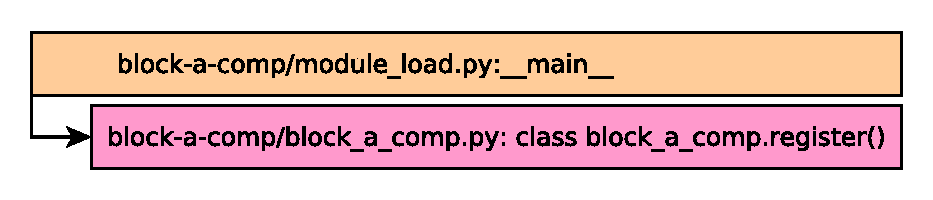
\includegraphics[width=\linewidth]{diagrams/init_load_module.pdf}
            }
        \end{minipage}
    \item[\cod{\circled{2}}] The same (substitute a$→$b).

    \item[\cod{\circled{3}}]
        Note that \cod[magenta!35]{add_objects} adds normally pre-configured objects:
        \begin{minipage}[t]{\linewidth}
            \adjustbox{valign=t}{%
                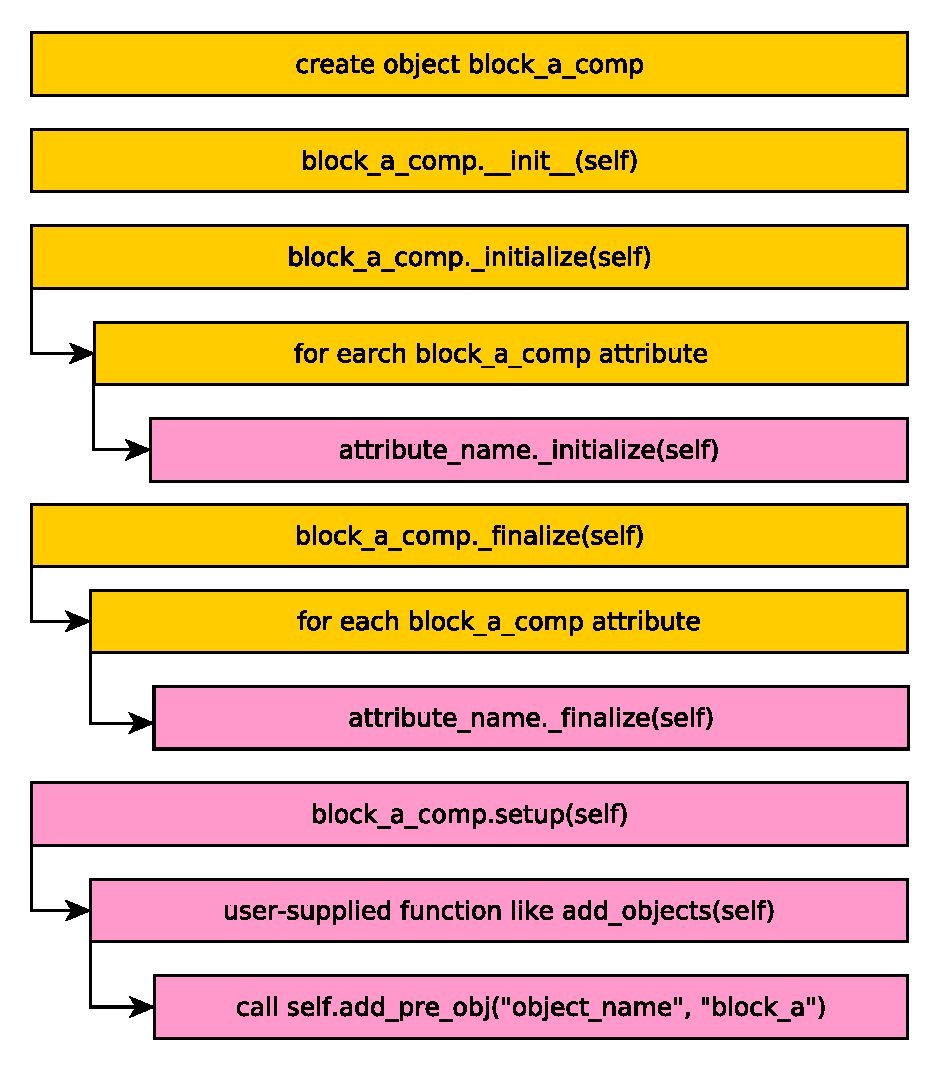
\includegraphics[width=\linewidth]{diagrams/init_create_comp.pdf}
            }
        \end{minipage}

    \item[\cod{\circled{4}}] The same (substitute a$→$b).

    \item[\cod{\circled{5}}]
        \begin{minipage}[t]{\linewidth}
            \adjustbox{valign=t}{%
                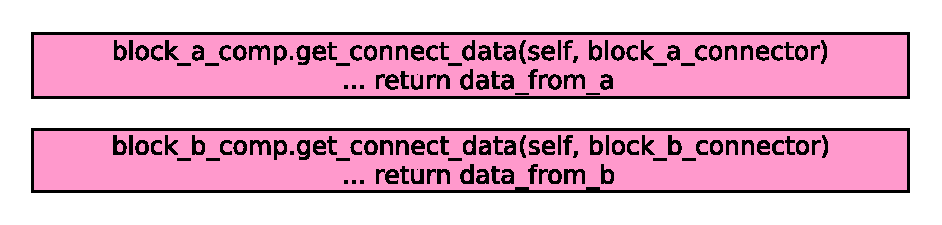
\includegraphics[width=\linewidth]{diagrams/init_connect.pdf}
            }
        \end{minipage}
        Note \cod[magenta!35]{get_connect_data} is basically just
        a \cod{switch/case} statement that chooses which data (object
        references, port names, etc) to pass to \cod[magenta!35]{connect}
        function call below.

    \item[\cod{\circled{6a}}]
        \begin{minipage}[t]{\linewidth}
            \adjustbox{valign=t}{%
                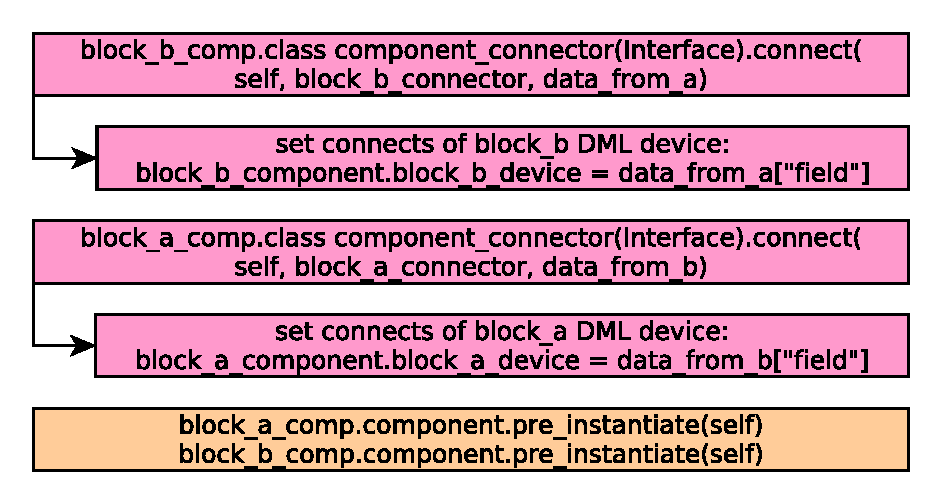
\includegraphics[width=\linewidth]{diagrams/init_instantiate_components.pdf}
            }
        \end{minipage}

    \item[\cod{\circled{6b}}]
        Pre-configuration ends and finally \cod{instantiate-components}
        begins to configure real DML objects:

        \begin{minipage}[t]{\linewidth}
            \adjustbox{valign=t}{%
                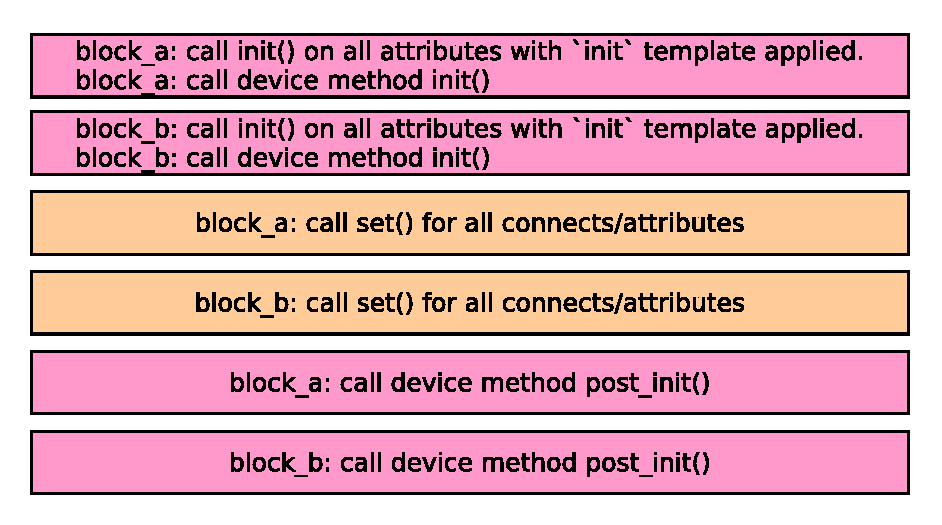
\includegraphics[width=\linewidth]{diagrams/init_instantiate_components_real_devices.pdf}
            }
        \end{minipage}

    \item[\cod{\circled{6c}}]
        Rarely some additional tweaks are required on real (already configured) device:

        \begin{minipage}[t]{\linewidth}
            \adjustbox{valign=t}{%
                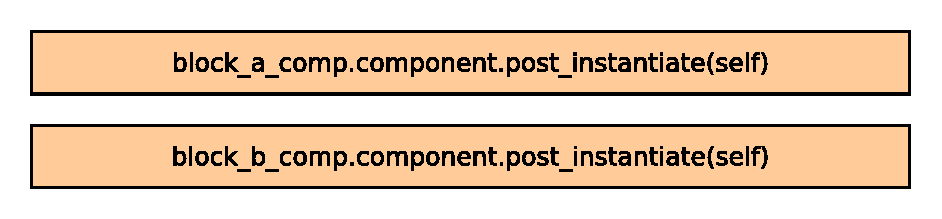
\includegraphics[width=\linewidth]{diagrams/init_instantiate_components_post.pdf}
            }
        \end{minipage}
\end{itemize}

Copyright \copyright\ 2021—2022 Andrey Makarov \\
\href{https://github.com/a-mr/simics-cheatsheet}{https://github.com/a-mr/simics-cheatsheet}
Version 0.2 (Simics 6.0.116)

\ifdefined\cheatsheetCompact
\end{multicols*}
\fi
\end{document}
